\documentclass[11pt]{article}
% Shared preamble of the RMC kernel write-ups (% Shared preamble of the RMC kernel write-ups (% Shared preamble of the RMC kernel write-ups (\input{preamble} after \documentclass).
\usepackage[margin=1in]{geometry}
\usepackage{amsmath,amssymb,bm}
\usepackage{graphicx}
\usepackage{booktabs}
\usepackage{hyperref}

\newcommand{\dd}{\,\mathrm{d}}
\newcommand{\Ein}{E}
\newcommand{\Eout}{E'}
\newcommand{\Ecm}{E_{c}}
\newcommand{\mucm}{\mu_{c}}
\newcommand{\mulab}{\mu_0}

% Common closing section: how the verification figures are produced
\newcommand{\verificationmethod}{%
Each figure is produced by \texttt{verification/verify\_laws.py}. For an incident
energy $\Ein$ along $+z$, $10^6$ collisions are sampled with MC/DC's own reaction
sampler (\texttt{sample\_elastic\_scattering}, \texttt{sample\_inelastic\_scattering}
or \texttt{sample\_fission}), and every emitted neutron is histogrammed in
$48 \times 24$ bins of $(\Eout, \mulab)$, with $\mulab$ the lab cosine to $+z$. The
inverted kernel used by RMC is integrated over the same bins (Gauss--Legendre panels;
two-body lines are split where $\mulab^*(\Eout)$ crosses a cosine edge), multiplied by
the number of collisions, and compared with a $\chi^2$ test over bins with at least 5
expected counts (the rest pooled into one bin). The tables list $\chi^2/\mathrm{dof}$,
its $p$-value, the emitted neutrons per collision (sampled vs.\ the integral of the
inverted kernel), and the largest relative change of a bin integral when the
quadrature panels are doubled. Left panels: outgoing-energy marginal; middle:
lab-cosine marginal; right: per-bin $z = (\text{sampled} - \text{inverted}) /
\sqrt{\text{inverted}}$.}
 after \documentclass).
\usepackage[margin=1in]{geometry}
\usepackage{amsmath,amssymb,bm}
\usepackage{graphicx}
\usepackage{booktabs}
\usepackage{hyperref}

\newcommand{\dd}{\,\mathrm{d}}
\newcommand{\Ein}{E}
\newcommand{\Eout}{E'}
\newcommand{\Ecm}{E_{c}}
\newcommand{\mucm}{\mu_{c}}
\newcommand{\mulab}{\mu_0}

% Common closing section: how the verification figures are produced
\newcommand{\verificationmethod}{%
Each figure is produced by \texttt{verification/verify\_laws.py}. For an incident
energy $\Ein$ along $+z$, $10^6$ collisions are sampled with MC/DC's own reaction
sampler (\texttt{sample\_elastic\_scattering}, \texttt{sample\_inelastic\_scattering}
or \texttt{sample\_fission}), and every emitted neutron is histogrammed in
$48 \times 24$ bins of $(\Eout, \mulab)$, with $\mulab$ the lab cosine to $+z$. The
inverted kernel used by RMC is integrated over the same bins (Gauss--Legendre panels;
two-body lines are split where $\mulab^*(\Eout)$ crosses a cosine edge), multiplied by
the number of collisions, and compared with a $\chi^2$ test over bins with at least 5
expected counts (the rest pooled into one bin). The tables list $\chi^2/\mathrm{dof}$,
its $p$-value, the emitted neutrons per collision (sampled vs.\ the integral of the
inverted kernel), and the largest relative change of a bin integral when the
quadrature panels are doubled. Left panels: outgoing-energy marginal; middle:
lab-cosine marginal; right: per-bin $z = (\text{sampled} - \text{inverted}) /
\sqrt{\text{inverted}}$.}
 after \documentclass).
\usepackage[margin=1in]{geometry}
\usepackage{amsmath,amssymb,bm}
\usepackage{graphicx}
\usepackage{booktabs}
\usepackage{hyperref}

\newcommand{\dd}{\,\mathrm{d}}
\newcommand{\Ein}{E}
\newcommand{\Eout}{E'}
\newcommand{\Ecm}{E_{c}}
\newcommand{\mucm}{\mu_{c}}
\newcommand{\mulab}{\mu_0}

% Common closing section: how the verification figures are produced
\newcommand{\verificationmethod}{%
Each figure is produced by \texttt{verification/verify\_laws.py}. For an incident
energy $\Ein$ along $+z$, $10^6$ collisions are sampled with MC/DC's own reaction
sampler (\texttt{sample\_elastic\_scattering}, \texttt{sample\_inelastic\_scattering}
or \texttt{sample\_fission}), and every emitted neutron is histogrammed in
$48 \times 24$ bins of $(\Eout, \mulab)$, with $\mulab$ the lab cosine to $+z$. The
inverted kernel used by RMC is integrated over the same bins (Gauss--Legendre panels;
two-body lines are split where $\mulab^*(\Eout)$ crosses a cosine edge), multiplied by
the number of collisions, and compared with a $\chi^2$ test over bins with at least 5
expected counts (the rest pooled into one bin). The tables list $\chi^2/\mathrm{dof}$,
its $p$-value, the emitted neutrons per collision (sampled vs.\ the integral of the
inverted kernel), and the largest relative change of a bin integral when the
quadrature panels are doubled. Left panels: outgoing-energy marginal; middle:
lab-cosine marginal; right: per-bin $z = (\text{sampled} - \text{inverted}) /
\sqrt{\text{inverted}}$.}


\title{Inverted kernel: N-body phase-space distribution (ENDF Law 6 / ACE Law 66)}
\date{}

\begin{document}
\maketitle

\noindent Code: \texttt{evaluate\_nbody}, \texttt{nbody\_energy\_max} in
\texttt{mcdc/rmc/evaluate.py}; MC/DC: \texttt{DistributionNBody},
\texttt{\_sample\_correlated\_distribution}.

\section{The law}

For $n$ emitted particles of total mass ratio $A_p$ (to the neutron), the COM energy
of one emitted neutron follows the phase-space density
\begin{equation}
  P(\Ecm \mid \Ein) = C_n\,\sqrt{\Ecm}\,\big(E_{\max} - \Ecm\big)^{3n/2 - 4},\qquad
  E_{\max}(\Ein) = \frac{A_p - 1}{A_p}\left(\frac{A}{A+1}\Ein + Q\right),
\end{equation}
with an isotropic COM cosine. ACE stores the distribution of the reduced variable
$T = \Ecm/E_{\max} \in [0, 1]$ as a linear table $\{T_k, p_k\}$ together with $n$
(NPSX) and $A_p$.

\section{What MC/DC samples (after the fix)}

The data generator previously dropped $n$ and $A_p$ and stored $T$ as an energy in MeV,
so MC/DC returned $T\times 1$\,MeV whatever the incident energy. With
\texttt{fix/free-gas-temperature-nbody-scaling} the generator stores
\texttt{number\_of\_particles} and \texttt{total\_mass\_ratio}, the distribution
carries $E_{\max}(\Ein) = s\,\Ein + o$ with $s = (A_p - 1)A/(A_p(A+1))$ and
$o = (A_p - 1)Q/A_p$, and the sampler returns
\begin{equation}
  T \sim p(T)\ \text{(exact inversion of the linear table)},\qquad
  \Ecm = T\,E_{\max}(\Ein),\qquad \mucm \sim U(-1, 1).
\end{equation}

\section{Inverted kernel}

Changing variables from $T$ to $\Ecm$,
\begin{equation}
  f_C(\Ecm, \mucm \mid \Ein) = \frac{p\big(\Ecm/E_{\max}\big)}{E_{\max}}\cdot\frac12,
  \qquad 0 \le \Ecm \le E_{\max}(\Ein),
\end{equation}
zero for $E_{\max} \le 0$ (below threshold), and $f_L = Y f_C\sqrt{\Eout/\Ecm}$. The
table points $T_k E_{\max}$ are the breakpoints of the energy density. For H-2 MT-16,
$n = 3$ and $A_p = 2.9986$, so the exact law is
$\sqrt{\Ecm}\,(E_{\max} - \Ecm)^{1/2}$; its square-root endpoints make the bin
quadrature converge more slowly than for the other laws (the quadrature column in the
table), still far below the statistical error.

\section{Verification}
\verificationmethod

\begin{center}
\begin{tabular}{rrrrrrr}
\toprule
$E$ [eV] & samples & bins & $\chi^2/\mathrm{dof}$ & $p$ & yield (sampled / inverted) & quad. err. \\
\midrule
8e+06 & 1e+06 & 394 & 418.7/394 & 0.188 & 2.00000 / 2.00000 & 4.7e-03 \\
1.8e+07 & 1e+06 & 458 & 425.3/458 & 0.861 & 2.00000 / 2.00000 & 1.9e-03 \\
\bottomrule
\end{tabular}

\end{center}

\begin{figure}[h]
  \centering
  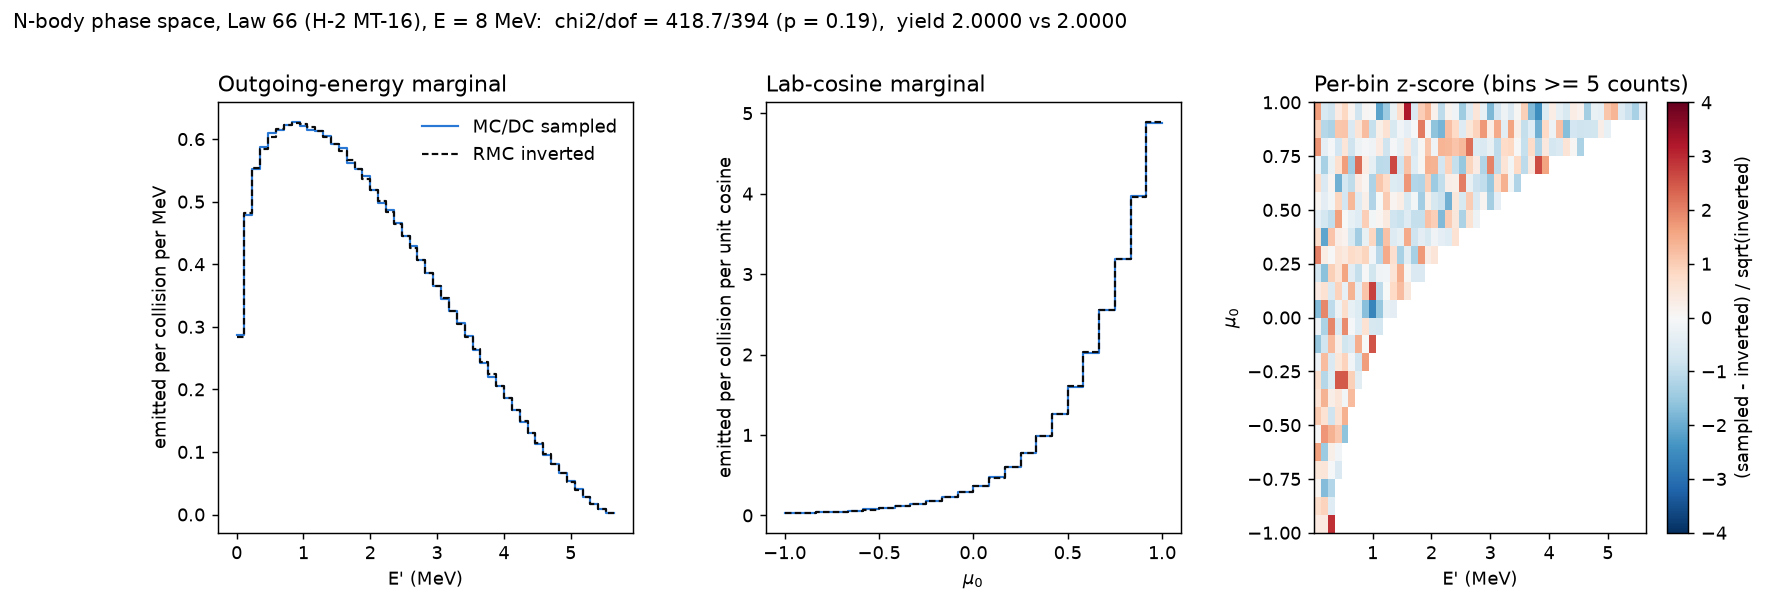
\includegraphics[width=\textwidth]{figures/n_body/n_body_E8e06.png}
  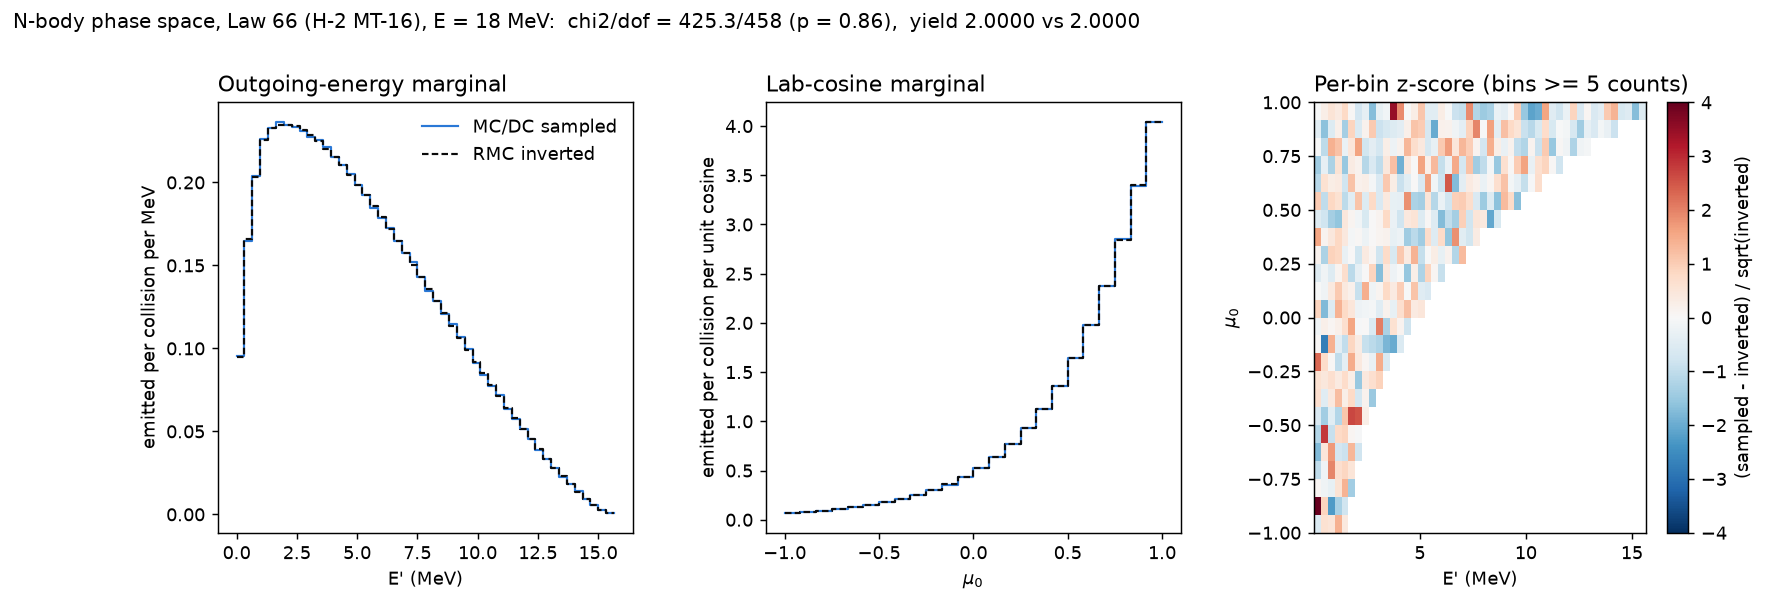
\includegraphics[width=\textwidth]{figures/n_body/n_body_E1p8e07.png}
  \caption{H-2 MT-16 $(n,2n)$, regenerated data, at 8 and 18\,MeV: two neutrons per
  collision, $E_{\max}$ growing with the incident energy.}
\end{figure}

\end{document}
